\subsection{Problema 2 - Probabilidade de Erro: \texorpdfstring{$M$}{M}-QAM}
Para calcular a probabilidade de erro $P(e)$ de cada constelação~\ref{eq:Pe_M_QAM} desenvolvida em~\cite{Cecilio}.
\begin{equation}
    P(e) = 4 \left(1-\frac{1}{\sqrt{M}}\right) Q\left(\sqrt{\frac{3}{M-1}\frac{E_s}{N_0}}\right) - 4\left(1-\frac{1}{\sqrt{M}}\right)^2 Q^2\left(\sqrt{\frac{3}{M-1}\frac{E_s}{N_0}}\right)
    \label{eq:Pe_M_QAM}
\end{equation}

Para valores mais elevados de \textit{SNR}, a equação da probabilidade do $M$-QAM pode ser reduzida para~\ref{eq:Pe_reduzida_M_QAM}, pois o segundo termo ao quadrado passa a ser irrelevante.
\begin{equation}
    P(e) = 4 \left(1-\frac{1}{\sqrt{M}}\right) Q\left(\sqrt{\frac{3}{M-1}\frac{E_s}{N_0}}\right)
    \label{eq:Pe_reduzida_M_QAM}
\end{equation}

Nas simulações realizadas, as curvas utilizando ambas as equações são bem semelhantes, principalmente para constelação 4-QAM, além de reduzir o custo computacional. Entretanto, para manter a fidedignidade do gráfico mostrado na~\ref{fig:Erro_Teorico_MQAM}, a probabilidade $P(e)$ é caculada a partir da equação completa~\ref{eq:Pe_M_QAM}.

\begin{figure}[!ht]
    \centering
    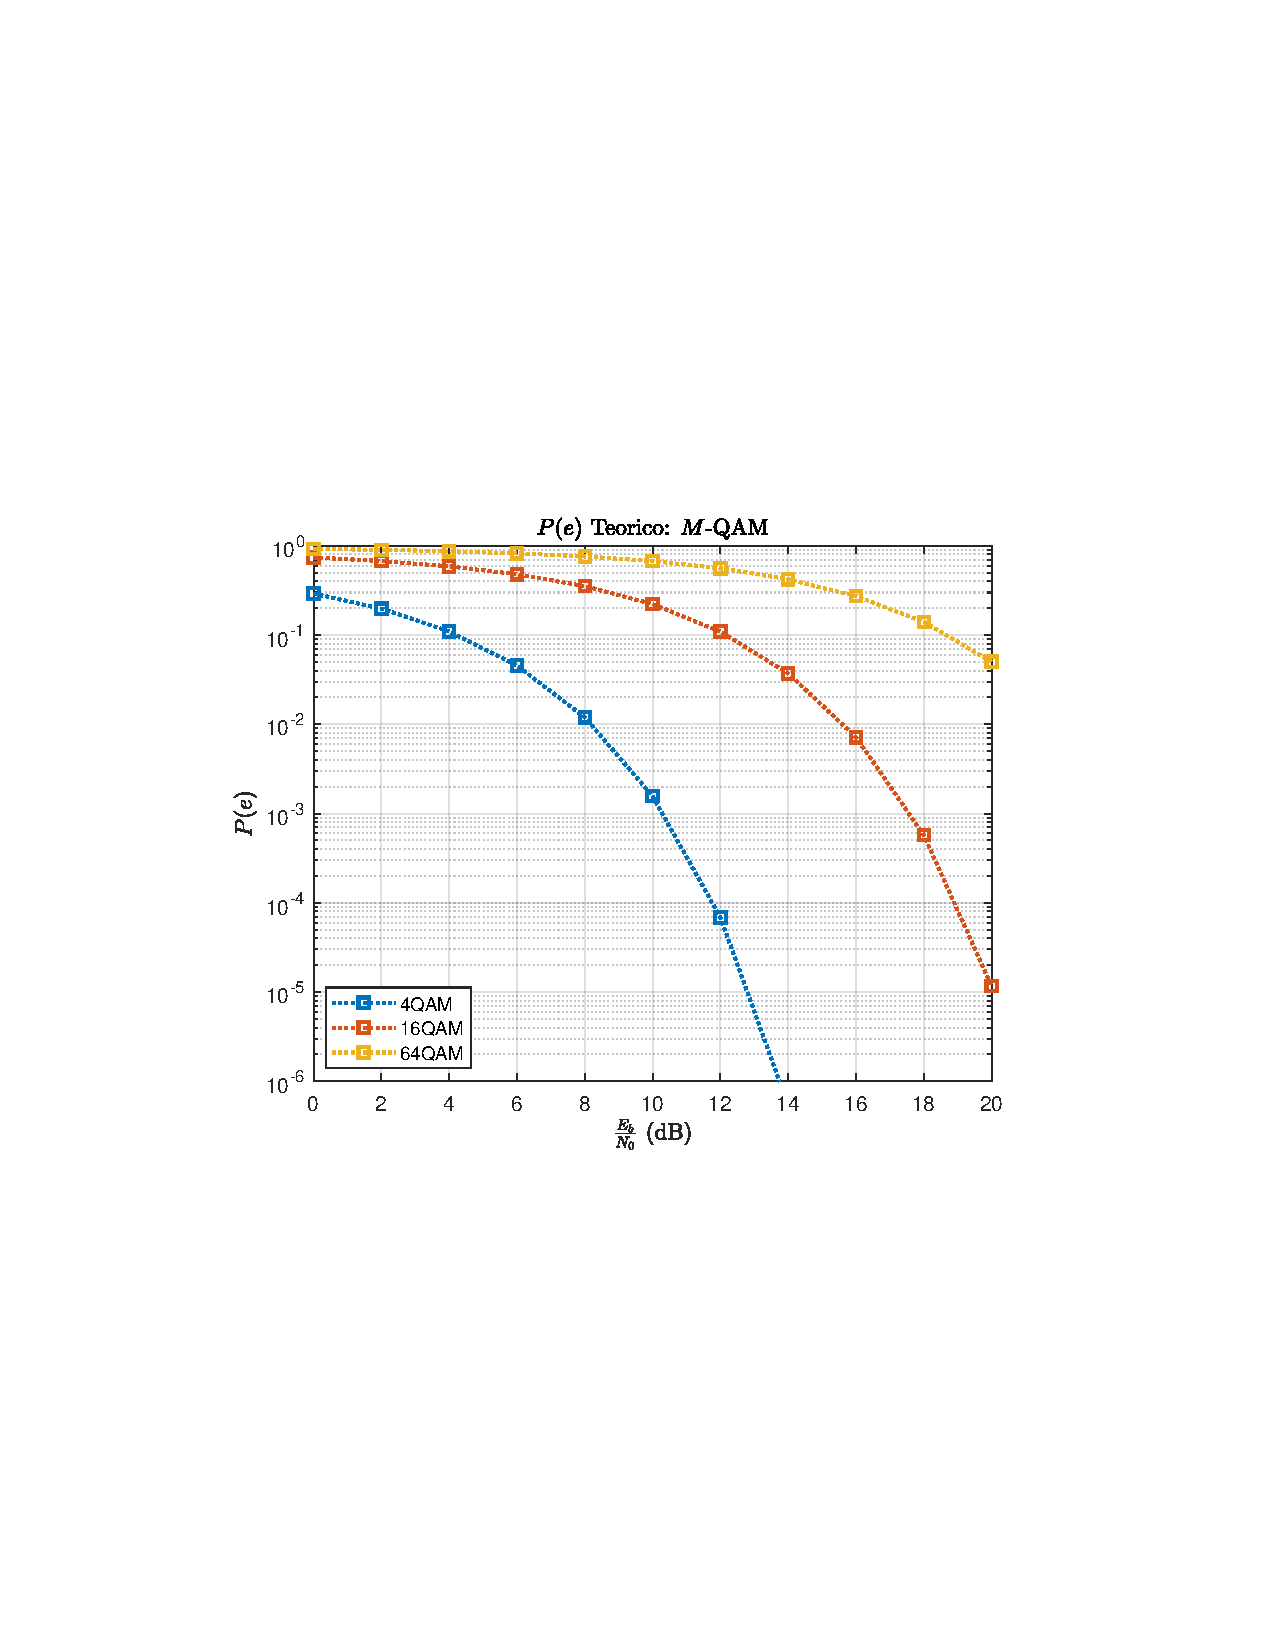
\includegraphics[width=1.0\textwidth,clip=true,trim={1.5cm 8.5cm 1.8cm 8.3cm}]{C:/Users/lukin/Documents/GitHub/Courses-HWs/Sistemas de Comunicacoes Digitais/matlab/problema2/fig/Erro_Teorico_MQAM.pdf}
    \caption{Probabilidade de erro $(P(e))$ teórico $M$-QAM.}
    \label{fig:Erro_Teorico_MQAM}
\end{figure}